%%%%%%%%%%%%%% 
% Fichero: EjFigs
% Autor: J. Salido (http://www.esi.uclm.es/www/jsalido)
% Fecha: febrero, 2017
% Descripción: Ejemplo básico de inclusión de figuras.
% Ejemplo del curso: “LaTeX esencial para preparación de TFG, Tesis
% y otros documentos académicos” (Esc. Sup. Informática-UCLM)
%%%%%%%%%%%%%%




%%%%%%%%%%%%%%
% Preámbulo del documento
%%%%%%%%%%%%%%
\documentclass[11pt,a4paper]{article} 
\usepackage[utf8]{inputenx} 
\usepackage[spanish]{babel} 
\usepackage[left=2cm,right=2cm,top=2cm,bottom=2cm]{geometry} % Márgenes 

% Tipografía
\usepackage{newpxtext}
\usepackage{newpxmath}

% Símbolos
\usepackage{marvosym}
\usepackage{pifont} % Generación de símbolos especiales
\usepackage{textcomp}

\usepackage[T1]{fontenc} % Codificación de salida    
\usepackage{microtype} % Mejoras de microtipografía en la obtención de PDF (sólo para pdflatex)

% Generación de hiperenlaces
\usepackage[pdftex,
	breaklinks,
	colorlinks, % OJO: Incompatible con paquete "menukeys"
	citecolor=blue, % Color de la citas
	urlcolor=blue, % Color de las URL
	bookmarksnumbered=true % Incluye números en bookmarks
    ]{hyperref}

\urlstyle{sf}


% Listas
\usepackage{paralist} % Mayor control de listas
\usepackage{multicol} % Elementos en varias columnas



% Gráficos
\usepackage{graphicx}  % Inclusión de figuras y escalado de cajas

% Declaración del path donde están los archivos de figuras. 
% También se puede incluir el path en el nombre del fichero.
\graphicspath{{../figs/}}  
\DeclareGraphicsExtensions{.pdf,.png,.jpg}
% Lista de extensiones de ficheros por orden de precedencia. De este modo no hace falta indicar la extensión del fichero y en caso de existir dos fichero con el mismos nombre y extensión diferente se emplea el que tiene una extensión con mayor prioridad.

\usepackage[margin=10pt,labelfont=bf]{caption}
\captionsetup[figure]{skip=5pt} % Necesario por si se desea colocar los títulos de las figs. en la parte superior. De este modo no queda tan pegado a la figura.

% Con estas instrucciones se ajustan los valores del índice
\setcounter{secnumdepth}{1} % Ajusta el valor del último nivel numerado
\setcounter{tocdepth}{2} %Ajusta el valor del último nivel que aparece en TOC


\author{Jesús Salido}
\title{Inclusión básica de figuras en \LaTeX{}}
\date{\today}

%%%%%%%%%%%%%%
% Comienzo del documento
%%%%%%%%%%%%%%
\begin{document}

\maketitle

\begin{abstract}
	Explicación introductoria sobre cómo se incluyen y manejan las figuras con \LaTeX{}.
\end{abstract}

\tableofcontents
\listoffigures


\section{Primeros pasos}
La inclusión de figuras y archivos de imagen en un documento elaborado con \LaTeX{} es muy sencilla y versátil (en la Fig.~\ref{fig:plazaCR} se muestra una fotografía en formato \texttt{.jpg} en color).\footnote{El título de la imagen también muestra cómo debe darse créditos al autor de la imagen si ésta no es de libre uso y tenemos permiso para usarla.} Hay que tener presente que el tipo de ficheros permitidos depende de si empleamos \texttt{latex} o \texttt{pdflatex},\footnote{En todo este curso asumimos que trabajaremos con \texttt{pdfltex} pues es más cómodo y siempre es posible utilizar la herramienta \texttt{epstopdf} para realizar la conversión de formatos.} ya que el primero sólo permite la inclusión de ficheros gráficos \texttt{.eps} mientras el segundo admite \texttt{.pdf}, \texttt{.png} y \texttt{.jpg}. Cuando la figura original presente un formato diferentes a los soportados será preciso emplear algún programa para realizar la conversión apropiada de formatos.



% Ejemplo:
% ============
\begin{figure}[hbt] % Véase los tags de ubicación (h)ere, (b)ottom, (t)op 
	\centering % Fig. centrada en la página
% 	EDITAR: En caso de requerir que el título aparezca en la parte superior de la figura.
%	\caption[Ejemplo de foto en formato jpg]{La Plaza Mayor (cortesía de J.~Salido)} % Título y el título para la lista de figuras
	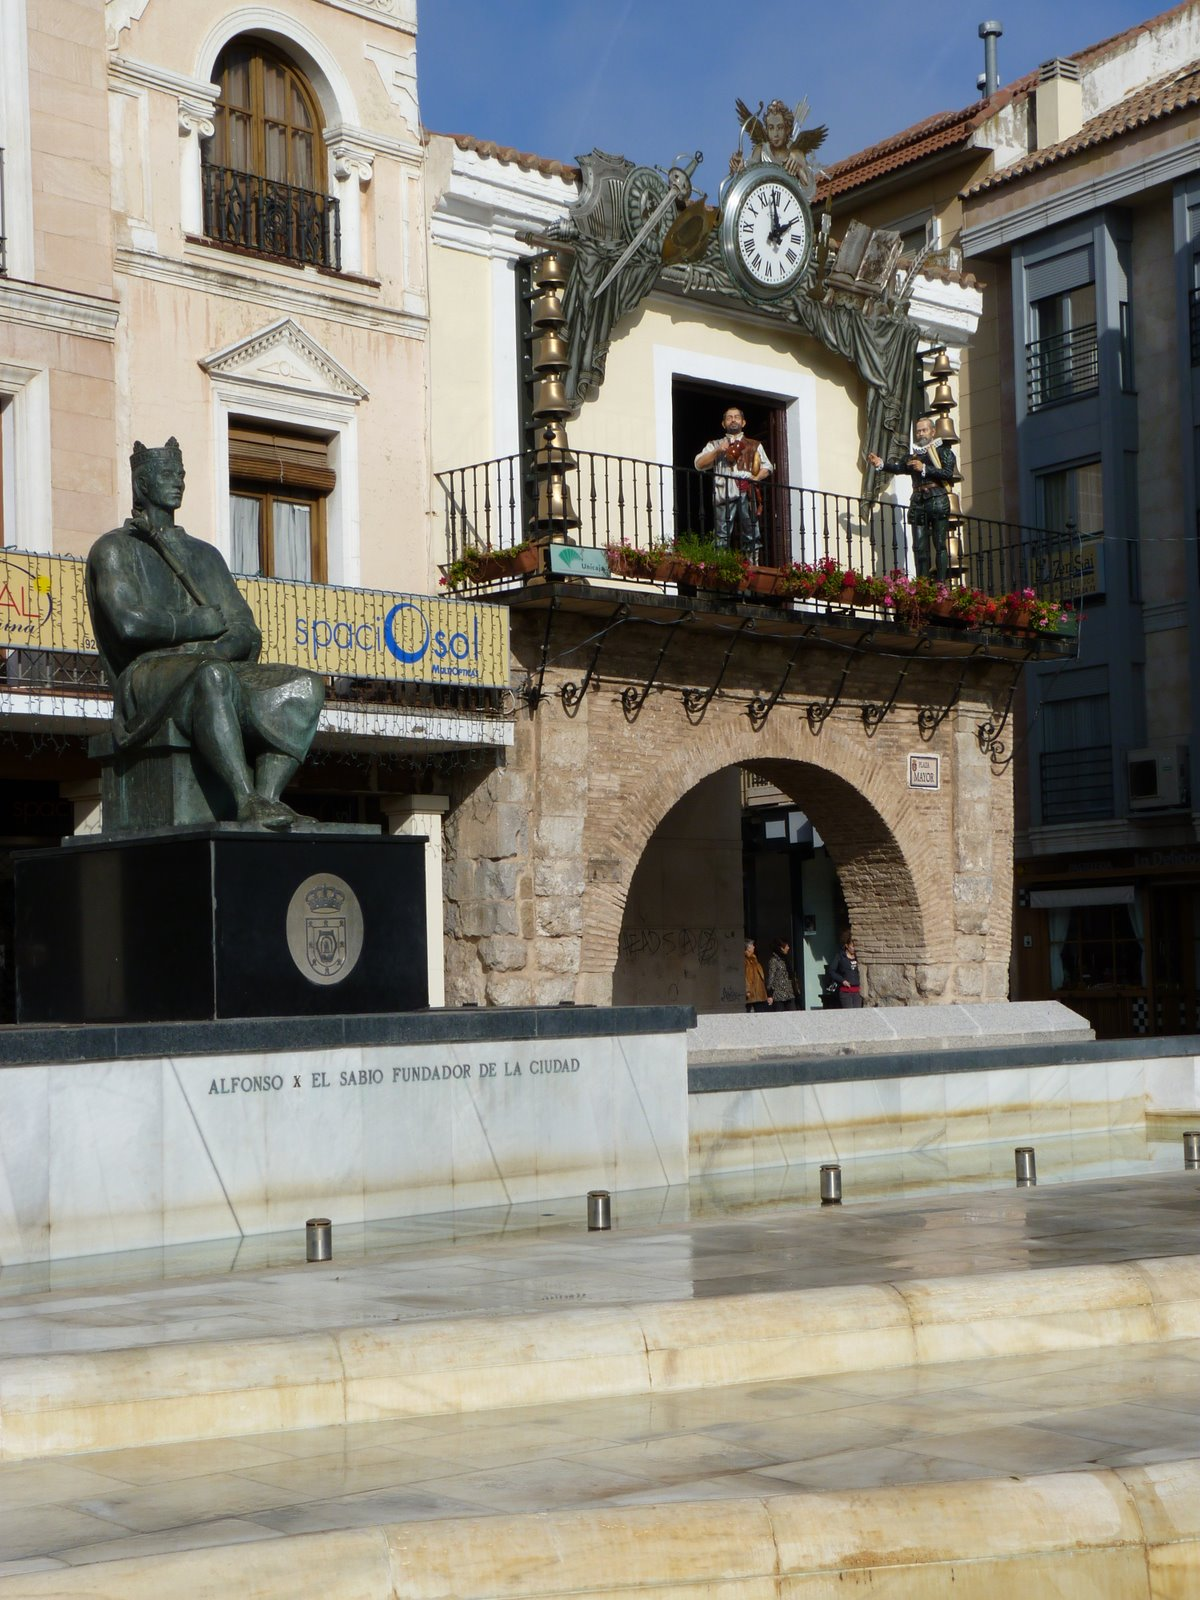
\includegraphics[height=6cm]{plazaCR} % Alto de la figura en la pág.
	\caption[Ejemplo de foto en formato jpg]{La Plaza Mayor (cortesía de J.~Salido)} % Título y el título para la lista de figuras
	\label{fig:plazaCR} % Etiqueta para las refs. cruzadas
\end{figure}


La inclusión de figuras requiere al menos el empleo del paquete \texttt{graphicx} con el que ya se pueden obtener resultados muy aceptables.

\LaTeX{} puede procesar las figuras como \emph{objetos deslizantes o <<flotantes>>}\footnote{Estos elementos se denominan \textit{float} y por ello a veces en español utilizamos como traducción <<flotante>>.} (o sin ubicación prefijada). De este modo \LaTeX{} emplea algoritmos para encontrar la mejor ubicación de todos los objetos flotantes que contenga el texto. El usuario siempre tiene a su disposición opciones para sugerir la ubicación deseada dejando a \LaTeX{} la reubicación del texto y párrafos en la página. Con todo, en ocasiones el usuario debe hacer algunos ajustes para conseguir la ubicación deseada, aunque sigue siendo un procedimiento mucho más cómodo que en algunos de los procesadores de texto \textsc{wysiwyg} populares. Siempre que existan muchas figuras en el texto el ajuste del resultado final va a ser más complejo y requerirá mayor intervención humana.


Otra de las ventajas de \LaTeX{} es que las imágenes no están incrustadas en nuestro fichero fuente, sino que son ficheros aparte incluidos durante la compilación. De este modo la modificación de la figura no requiere la modificación del fichero fuente sino únicamente una nueva compilación.


\section{Formatos gráficos}
A la hora de incluir figuras se debe decidir qué formato es el más apropiado entre los disponibles, siguiendo las siguientes reglas:
\begin{itemize}
	\item Siempre que sea posible es preferible el formato \texttt{.pfd} ya que es vectorial (escalable), aunque por supuesto si el fichero contiene alguna imagen de mapa de bits, esta no será escalable (véase Fig.~\ref{fig:4004arch}).
	\item Las fotografías se incluirán en formato \texttt{.jpg} (véase Fig.~\ref{fig:plazaCR})
	\item Las capturas de pantalla o gráficos de gran contraste se deben incluir en formato \texttt{.png} (véase Fig.~\ref{fig:inkscape}). 
	\item Siempre que se tenga un fichero de imagen (mapa de bits) con un fondo blanco u otro color plano, debería intentarse transformar en una imagen con fondo transparente convirtiéndola al formato \texttt{.png}.
\end{itemize}


% Ejemplo:
% ============
\begin{figure}[hbt]
	\centering
	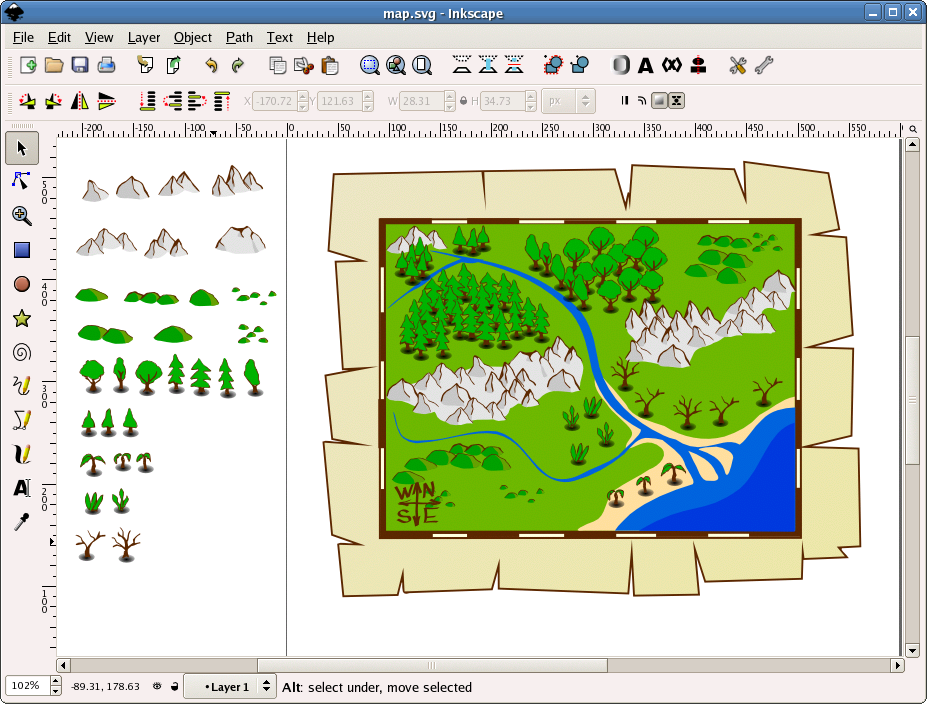
\includegraphics[width=0.4\linewidth]{inkscape} 
	\caption[Ejemplo de captura en png]{Captura de pantalla de \textsf{Inkscape}}
	\label{fig:inkscape}
\end{figure}

Las capturas de pantalla de programas deberían incluirse como ficheros en formato \texttt{.png}. En la Fig.~\ref{fig:inkscape} se muestra una captura del programa de libre distribución \textsf{InkScape}. Dicho programa es apropiado para la elaboración de gráficos vectoriales. 

% Ejemplo:
% ============
\begin{figure}[hbt]
	\centering
	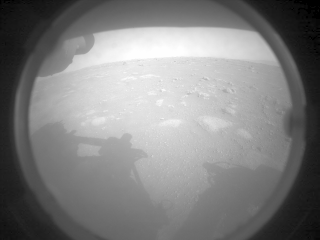
\includegraphics[width=0.6\linewidth]{Mars_Perseverance} 
	\caption[Foto histórica enviada desde Marte]{Primera foto enviada desde Marte el {18-2-2021} por el robot Perseverance (cortesía de NASA/JPL-Caltech)}
	\label{fig:inkscape}
\end{figure}


Siempre que sea posible emplear formato \texttt{.pdf} es preferible, ya que se trata de un formato vectorial con posibilidad de escalado sin pérdida de resolución. En la Fig.~\ref{fig:4004arch} se muestra el resultado de la inclusión de un gráfico en formato PDF. 

% Ejemplo:
% ============
\begin{figure}[hbt]
	\centering 
	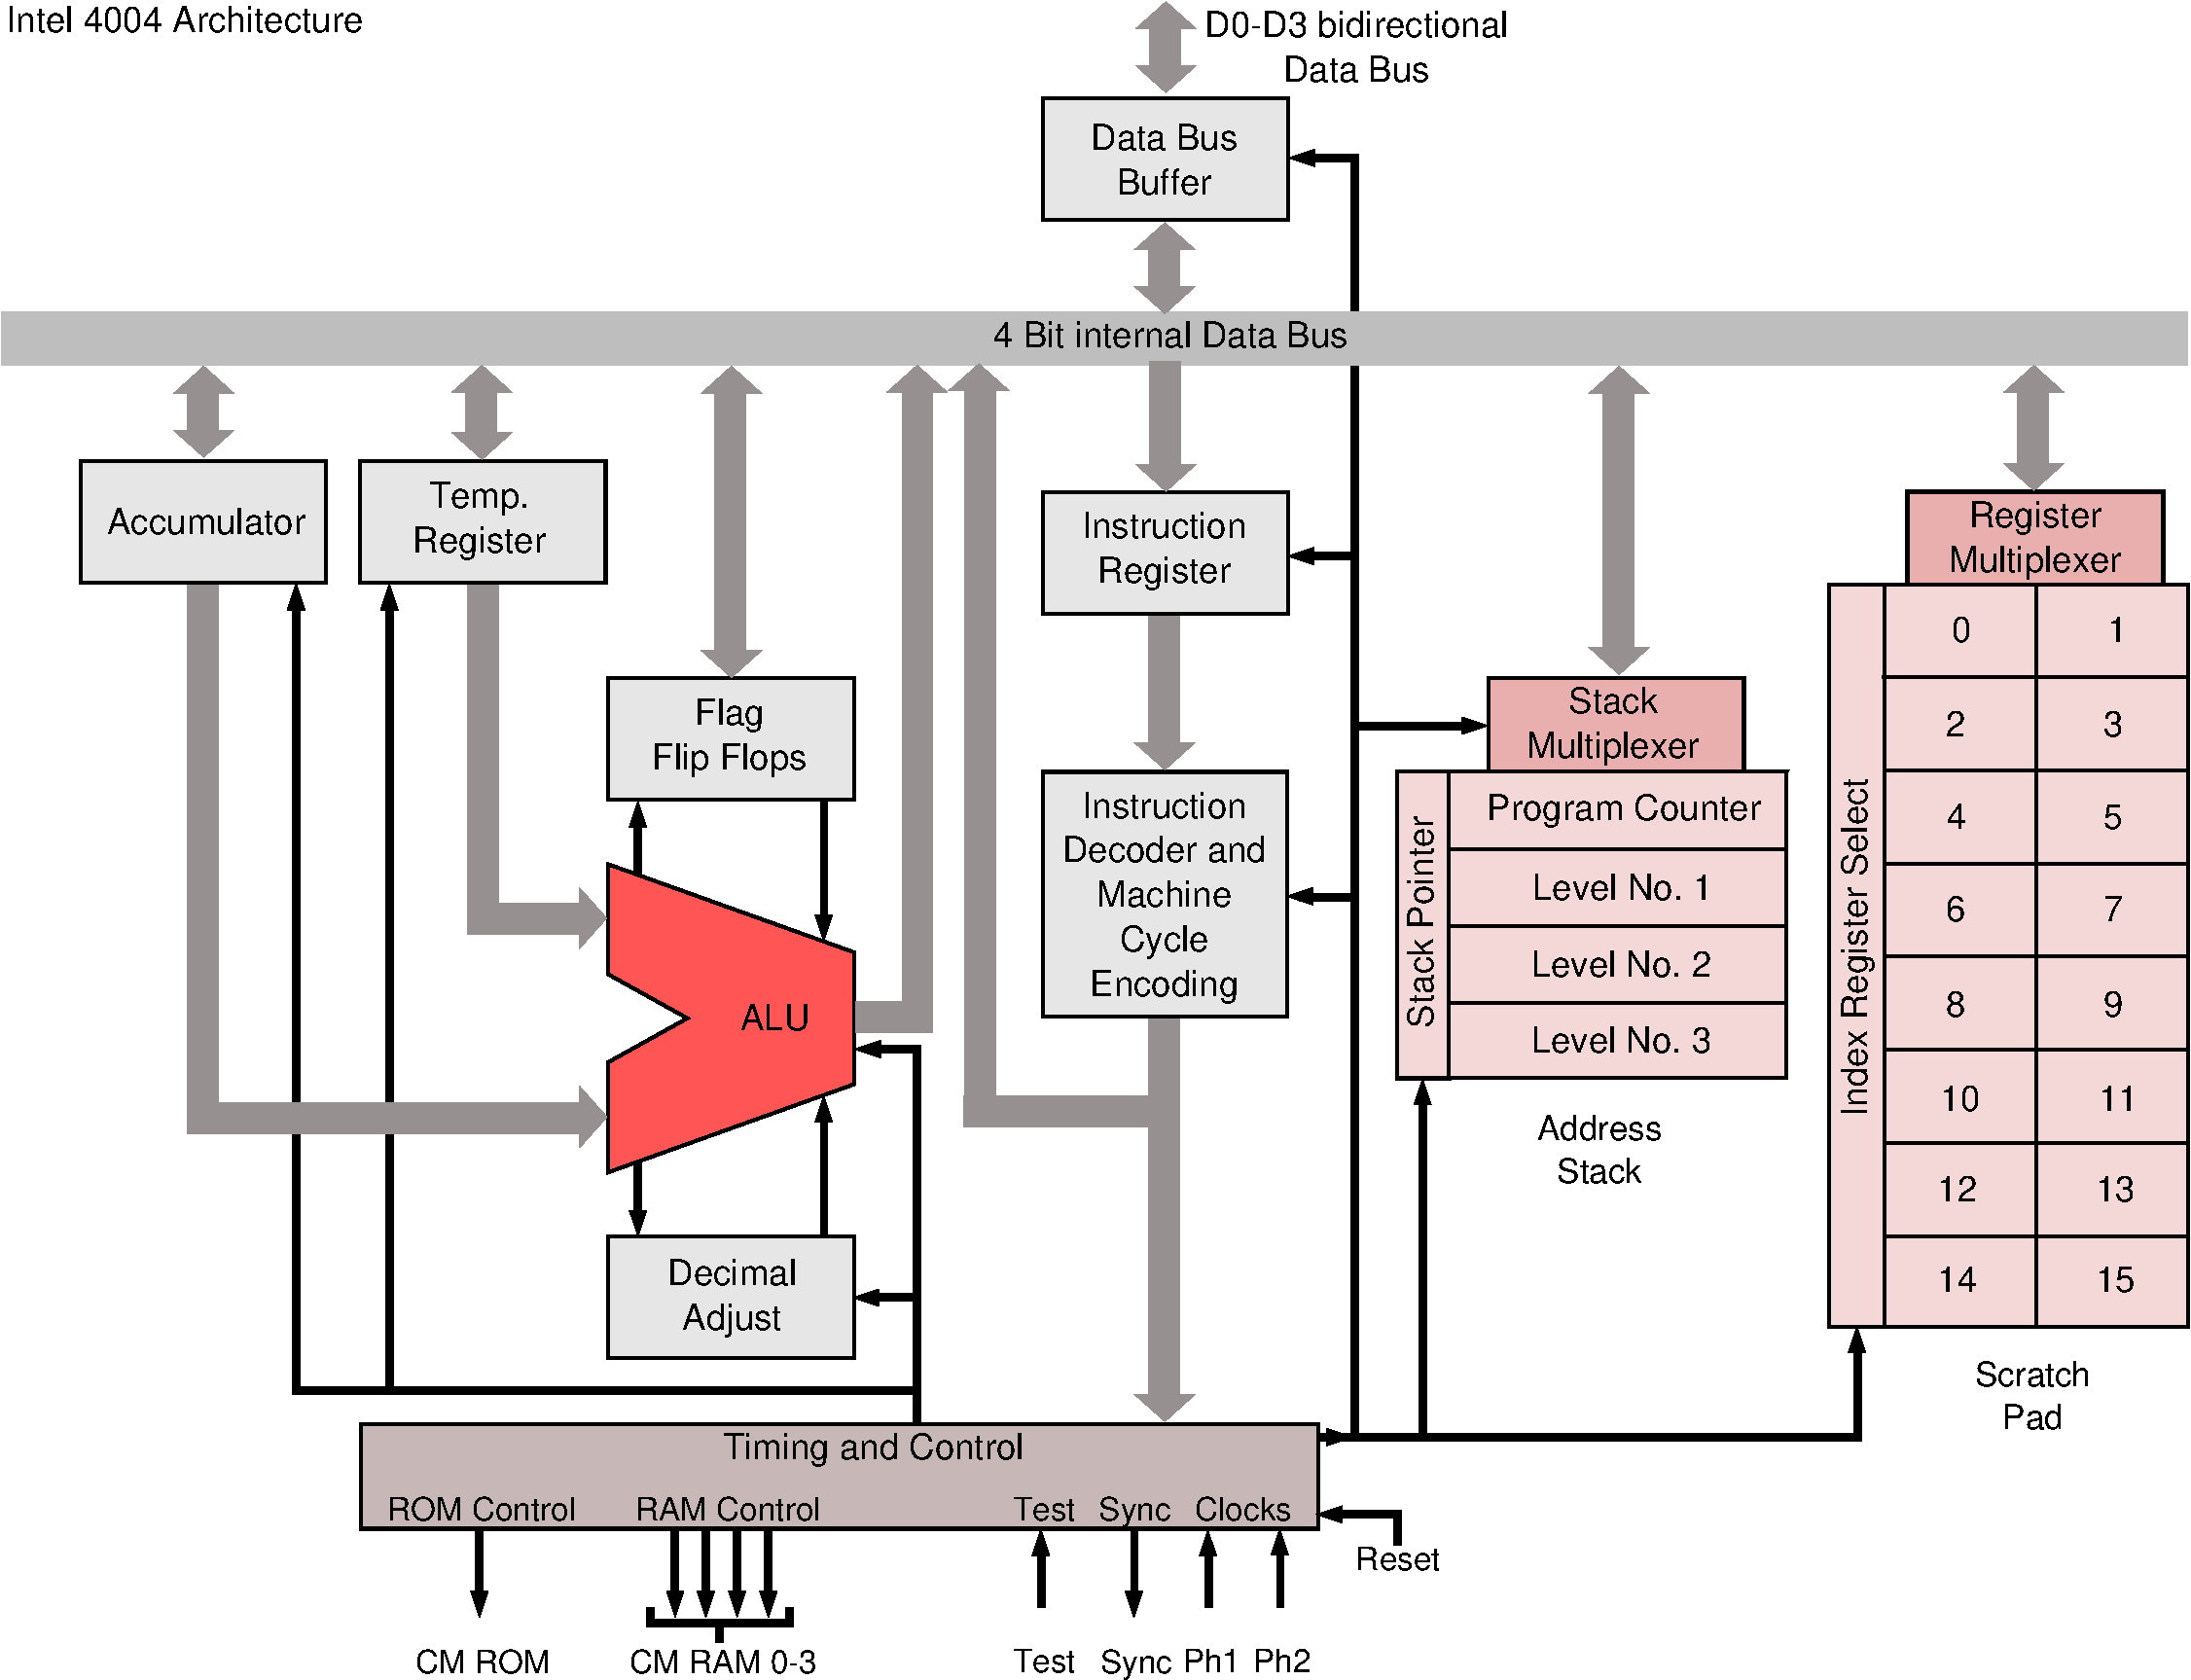
\includegraphics[width=0.5\linewidth]{4004arch} 
	\caption[Ejemplo de gráfico vectorial PDF]{Figura vectorial de arquitectura Intel 4004 (Wikimedia Commons)}
	\label{fig:4004arch}
\end{figure}


\subsection{Ventajas del formato PDF}
Una de las dificultades de trabajar con ficheros PDF es que se trata de un formato difícil de editar de modo que habitualmente se genera a partir de otros formatos. Por ejemplo, el gráfico de la Fig.~\ref{fig:4004arch}, cuyo formato original es \texttt{.svg}, ha sido realizado con el programa \textsf{InkScape} y convertido al formato PDF mediante la herramienta de exportación (a través de \textsf{Cairo}) incluida en el programa. En los programas que no incorporan dicha herramienta el fichero PDF se puede generar imprimiendo a un archivo con un driver de impresión PDF (si no se dispone del driver de Adobe se recomienda el uso de \textsf{PDFCreator}). 

Cuando se trabaja con figuras hay que tener mucho cuidado con emplear imágenes de Internet sin tener la seguridad de los términos de uso de las mismas. Con mucha frecuencia, de forma inadvertida, se violan los derechos de uso incluso cometiendo un delito. Por este motivo recomiendo recurrir a librerías de dominio público que permiten el uso de las imágenes y \emph{clip arts} sin restricciones, como por ejemplo Open ClipArt,\footnote{\url{http://openclipart.org/}} la página de galerías en el sitio de Inkscape\footnote{\url{http://wiki.inkscape.org/wiki/index.php/Galleries}} y Wikimedia Commons.\footnote{\url{http://commons.wikimedia.org/}}



\newpage
\subsection{Gráficas matemáticas}
En muchas ocasiones es preciso recurrir a una gráfica matemática para reflejar o apoyar una idea. Existen numerosos programas que ayudan a realizar estas gráficas, en cualquiera de los casos siempre se empleará un formato vectorial (PDF) para incluir la gráfica en nuestro documento. Nunca debe hacerse mediante una captura de pantalla pues en este caso estaremos perdiendo mucha información al tratar como un mapa de bits algo que es un objeto matemático y por tanto independiente de su escala de representación.

\subsubsection{Gráficas generadas con Excel}
Uno de los programas más universales para la creación de gráficas matemáticas son las hojas de cálculo como Excel. La Fig.~\ref{fig:excel} muestra un ejemplo de figura vectorial generada con ayuda de dicho programa.

% Ejemplo:
% ============
\begin{figure}[hbt]
	\centering
	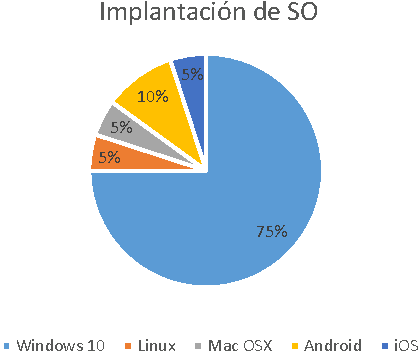
\includegraphics[width=0.5\linewidth]{EjFigsExcelOrig-crop} 
	\caption[Gráfico de Excel]{Figura vectorial generada con Excel}
	\label{fig:excel}
\end{figure}




\newpage
\subsubsection{Gráficas generadas con Matlab}
La Fig.~\ref{fig:matlabGrafs} muestra un ejemplo de figura vectorial generada con ayuda del programa Matlab. En este caso se observa cómo una única figura contiene distintos gráficos.

% Ejemplo:
% ============
\begin{figure}[hbt]
	\centering
	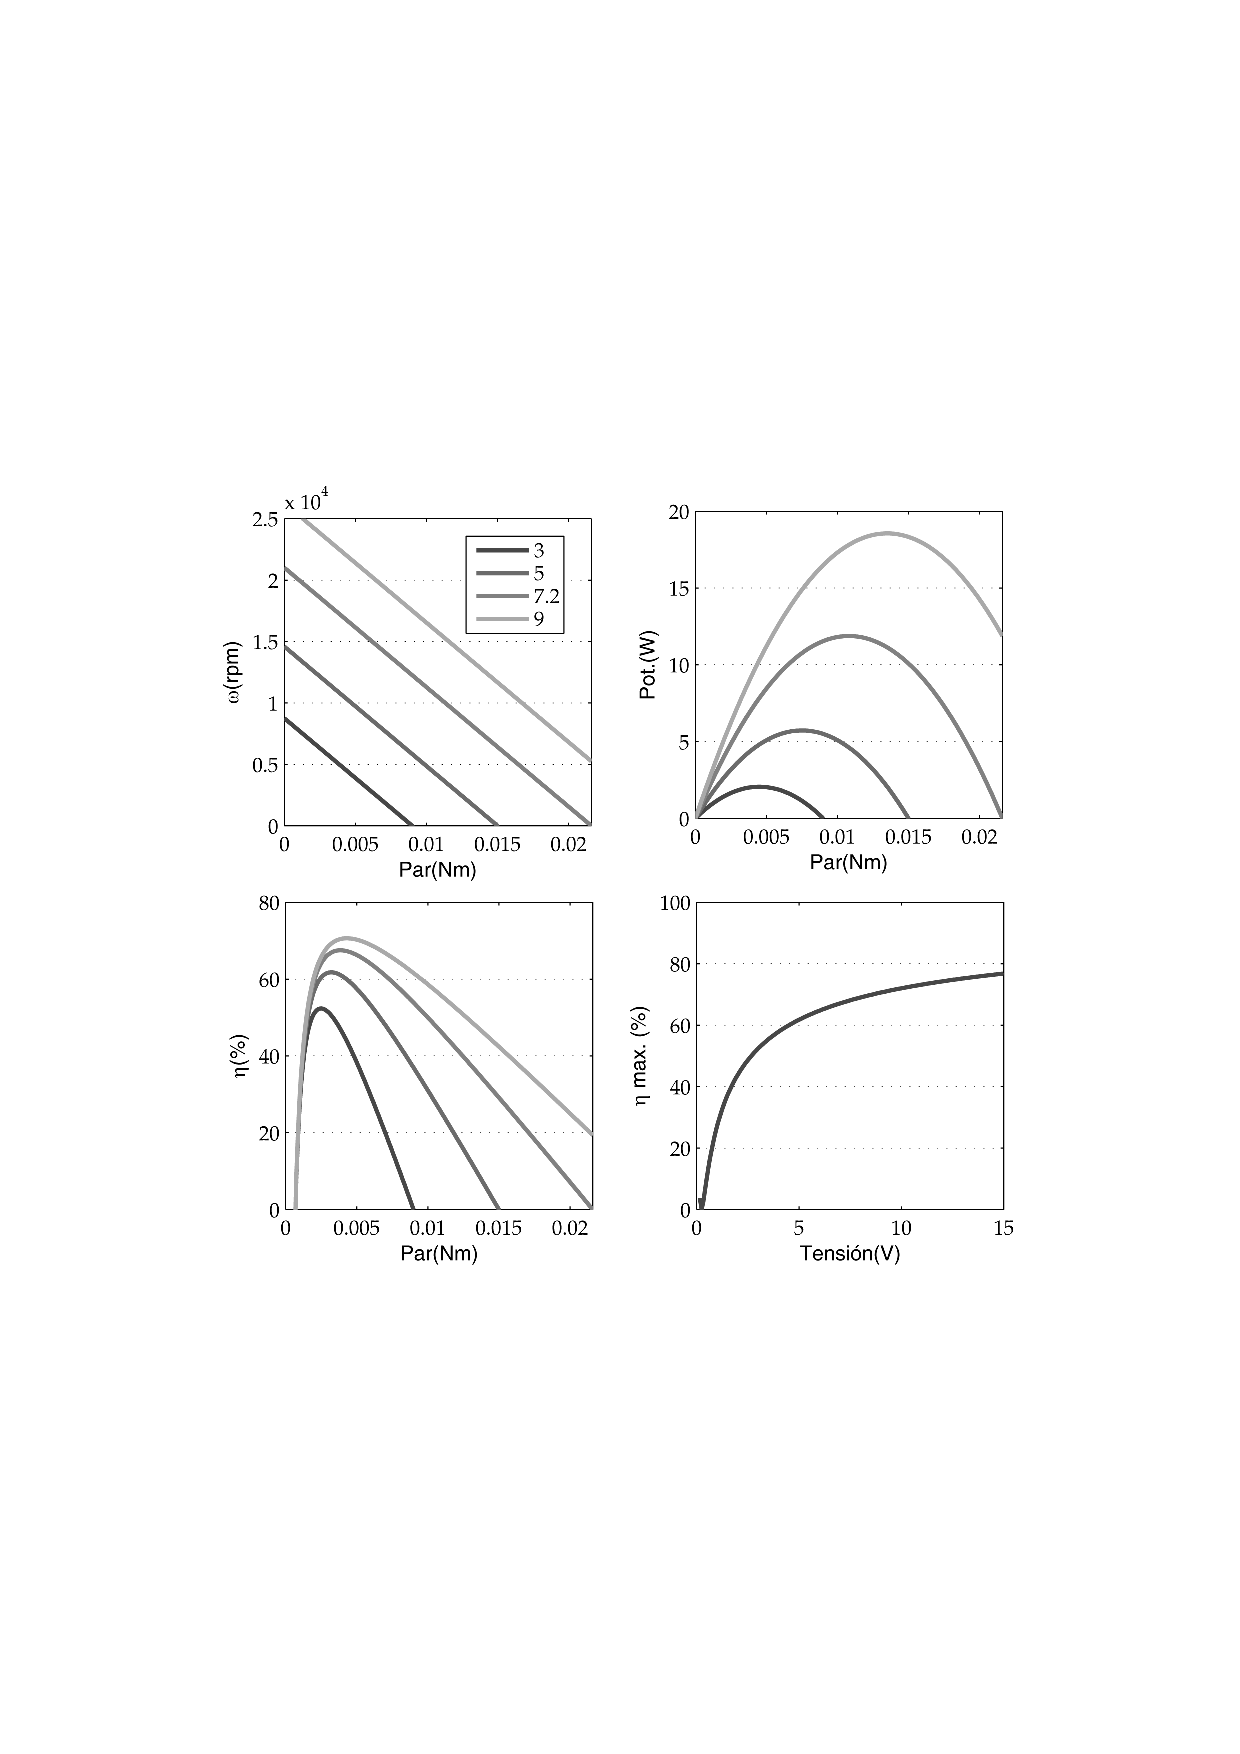
\includegraphics[width=0.8\linewidth]{matlabGrafs} 
	\caption[Gráfico de Matlab]{Figura vectorial generada con Matlab}
	\label{fig:matlabGrafs}
\end{figure}



\newpage
\subsubsection{Gráficas generadas con Matplotlib (Python)}
La Fig.~\ref{fig:python} muestra un ejemplo de figura vectorial (PDF) generada con Python y la librería \textsf{Matplotlib}. En este caso se observa cómo una única figura contiene distintos gráficos, siendo este un método alternativo al empleo de subfiguras.

% Ejemplo:
% ============
\begin{figure}[hbt]
	\centering
	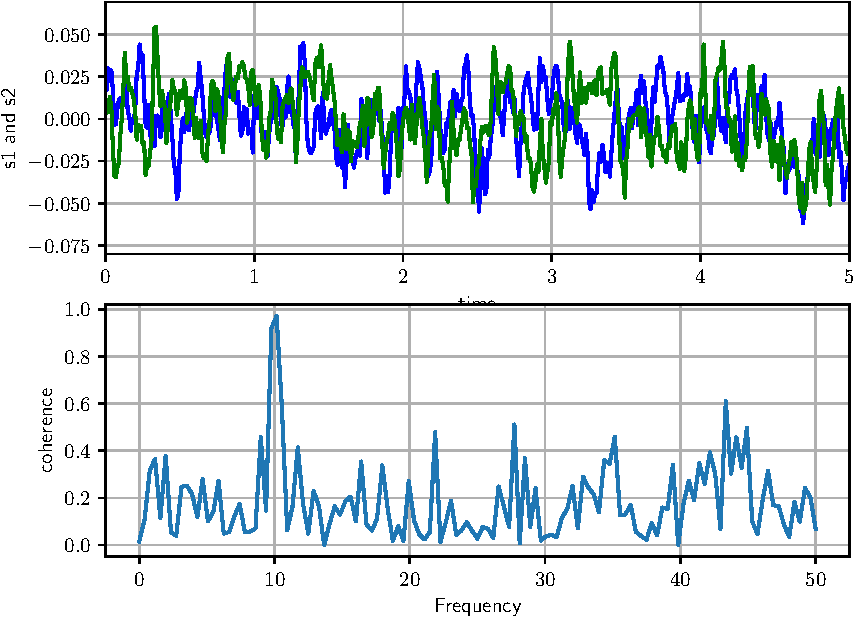
\includegraphics[width=0.8\linewidth]{fig2_py}
	\caption[Figura hecha desde Python]{Figura vectorial generada con Matplotlib (Python)}
	\label{fig:python}
\end{figure}


\subsection{Imágenes a las que se añaden gráficos}
En ocasiones es necesario recurrir a capturas de pantalla sobre las que es preciso realizar alguna anotación gráfica, por ejemplo añadiendo flechas y bloques de texto. Este es un caso que puede aparecer cuando se explica el funcionamiento de un programa informático (p.~ej.\ un manual). La captura siempre se debe realizar al mayor tamaño posible sobre la pantalla y se debe salvar en formato \texttt{.png}. Generalmente las herramientas de captura permiten la edición de la captura añadiéndole elementos gráficos e incluso texto. En este caso los elementos añadidos 
forman parte del fichero \texttt{.png} y por tanto son definidos como mapa de bits. Si se desea mantener las características escalables de los elementos gráficos, éstos deben ser añadidos mediante algún programa de edición vectorial (p.~ej.\ 
\textsf{Inkscape}, \textsf{Dia}, \textsf{Visio}, etc.) y salvar el fichero resultante en formato \texttt{.pdf}. Las figs.~\ref{fig:texmk02} y \ref{fig:texmk03} muestran las diferencias en los dos procesos mencionados.

% Ejemplo:
% ============
\begin{figure}[hbt]
	\centering
	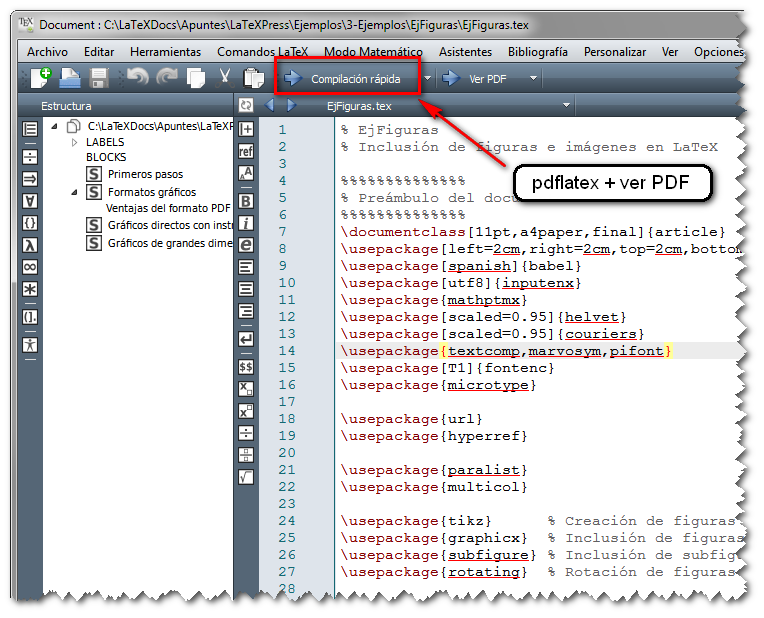
\includegraphics[width=0.5\textwidth]{texmk02} 
	\caption[Captura con gráfico en \texttt{png}]{Captura de pantalla con añadido gráfico en formato \texttt{png}}
	\label{fig:texmk02}
\end{figure}

% Ejemplo:
% ============
\begin{figure}[hbt]
	\centering
	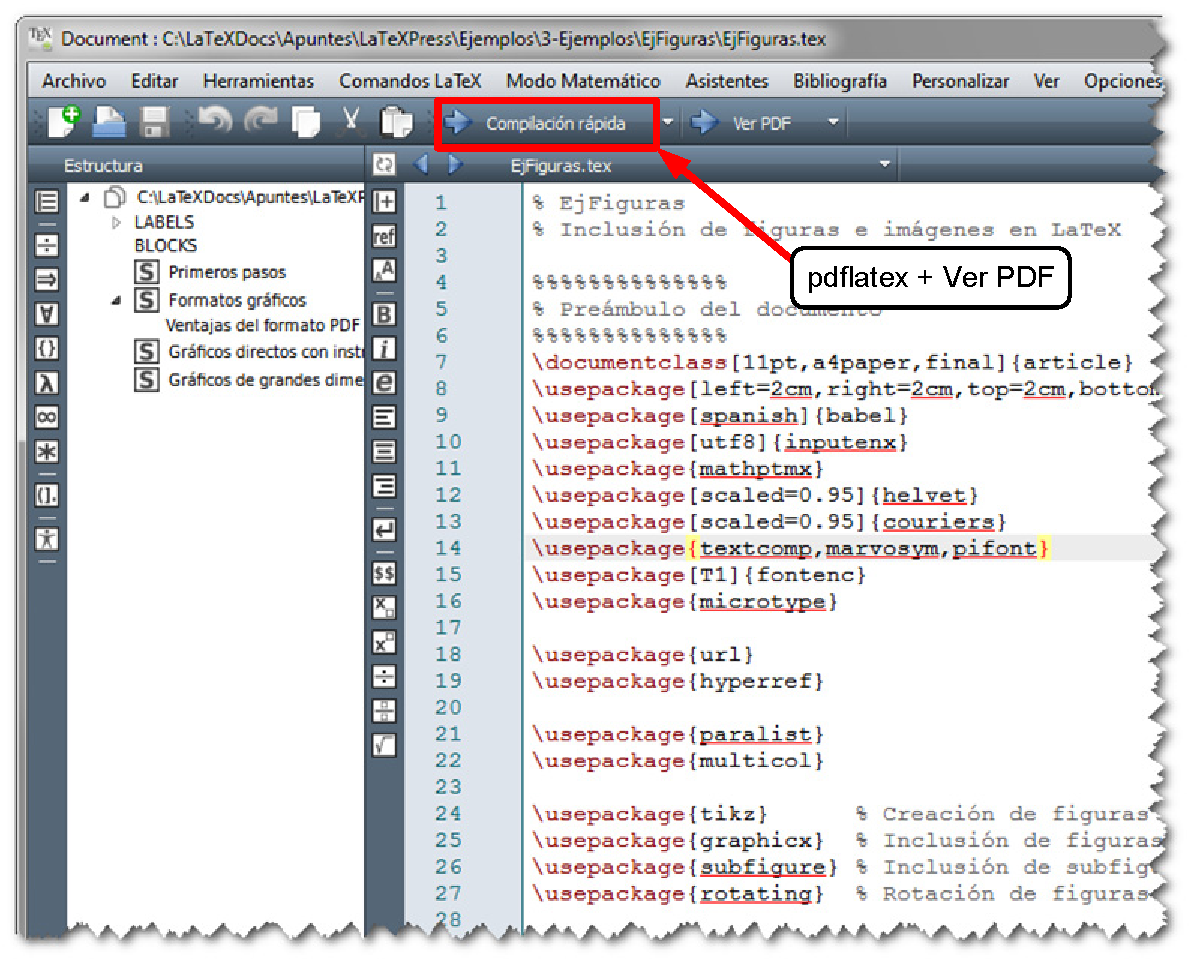
\includegraphics[width=0.5\textwidth]{texmk03} 
	\caption[Captura con gráfico en \texttt{pdf}]{Captura de pantalla con añadido gráfico en formato \texttt{pdf}}
	\label{fig:texmk03}
\end{figure}


\end{document}